\documentclass[conference]{IEEEtran}
\usepackage[T1]{fontenc}
\usepackage[utf8]{inputenc}
\usepackage{cite}
\usepackage{amsmath,amssymb,amsfonts}
\usepackage{graphicx}
\usepackage{textcomp}
\usepackage{xcolor}
\usepackage{booktabs}
\usepackage{array}
\usepackage{url}
\graphicspath{{figures/}}
\DeclareUnicodeCharacter{223C}{\ensuremath{\sim}}
\DeclareUnicodeCharacter{2208}{\ensuremath{\in}}
\DeclareUnicodeCharacter{2264}{\ensuremath{\leq}}
\DeclareUnicodeCharacter{2265}{\ensuremath{\geq}}
\DeclareUnicodeCharacter{2286}{\ensuremath{\subseteq}}
\DeclareUnicodeCharacter{2192}{\ensuremath{\to}}
\DeclareUnicodeCharacter{2212}{-}
\DeclareUnicodeCharacter{2203}{\ensuremath{\exists}}
\DeclareUnicodeCharacter{2200}{\ensuremath{\forall}}
\DeclareUnicodeCharacter{2227}{\ensuremath{\wedge}}
\DeclareUnicodeCharacter{2228}{\ensuremath{\vee}}
\DeclareUnicodeCharacter{21D2}{\ensuremath{\Rightarrow}}
\DeclareUnicodeCharacter{2260}{\ensuremath{\neq}}
\DeclareUnicodeCharacter{03A3}{\ensuremath{\Sigma}}
\DeclareUnicodeCharacter{0398}{\ensuremath{\Theta}}
\DeclareUnicodeCharacter{03B8}{\ensuremath{\theta}}
\DeclareUnicodeCharacter{03A0}{\ensuremath{\Pi}}
\DeclareUnicodeCharacter{03C4}{\ensuremath{\tau}}
\DeclareUnicodeCharacter{03C6}{\ensuremath{\varphi}}
\DeclareUnicodeCharacter{03A6}{\ensuremath{\Phi}}
\DeclareUnicodeCharacter{03B2}{\ensuremath{\beta}}
\DeclareUnicodeCharacter{03C1}{\ensuremath{\rho}}
\def\BibTeX{{\rm B\kern-.05em{\sc i\kern-.025em b}\kern-.08em
    T\kern-.1667em\lower.7ex\hbox{E}\kern-.125emX}}
\begin{document}
\title{MPTA-Repair: Multi-Property Clock-Bound Repair for Industrial Timed Automata}
\author{%
% TODO: Add the non-anonymous author names, affiliations, city/country, and email/ORCID. The Markdown-converted draft had an empty \author{} block.
}
\maketitle
\begin{abstract}
Timed automata are widely used to model and verify real-time systems with strict timing requirements. Industrial models are often checked against multiple predefined properties, including timed safety properties. When these properties are violated, the faults may stem from erroneous clock bounds in guards or invariants; however, repairing such bounds is challenging because a local change may affect other properties or alter intended untimed behavior. This paper presents MPTA-Repair, a counterexample-guided iterative approach for multi-property clock-bound repair of timed automata. It extracts repairable bounds from guards and invariants, analyzes diagnostic counterexamples, and uses MaxSMT-based repair generation to synthesize small candidate edits. Each candidate is validated against the full property set and checked for admissibility to ensure functional equivalence. Experiments on UPPAAL and XtaBenchmarkSuite benchmarks show a 93\% repair success rate, while an industrial case-study dataset achieves 76\%.
\end{abstract}
\begin{IEEEkeywords}
Timed automata, multi-property repair, clock-bound repair, counterexample-guided repair
\end{IEEEkeywords}
\section{Introduction}
\label{sec:introduction}

Real-time industrial systems combine discrete control logic with
quantitative timing requirements. In railway control, communication
protocols, and aerospace scheduling
~\cite{basile2021unisig,lonn1997tdma,david2010herschel},
correctness depends not only on which actions occur, but also on whether
they occur within permitted time windows. The scope of this paper is
timed safety properties rather than unbounded liveness properties,
because deadlines, bounded waiting, alarm durations, and error-state
reachability describe finite executions whose violations are directly
observable during design and testing
~\cite{kolbl2019clock,vogel2022patterns}. Timed automata (TAs) model
such behavior with clocks, guards, resets, and invariants
~\cite{alur1994theory,bengtsson2004timed}; practical systems are often
modeled as networks of timed automata (NTA).

Clock behavior is central to timed safety verification. Clocks and their
constraints encode deadlines, timeouts, durations, and delays. An
incorrect numerical bound in a transition guard or location invariant can
make otherwise valid discrete behavior occur too early, too late, or for
an invalid duration
~\cite{kolbl2019clock,jiang2010heart,lonn1997tdma}. This paper studies
clock-bound repair for NTA models, modifying only numerical bounds in
guards and invariants while leaving properties, locations, transitions,
synchronizations, clock references, resets, and data updates unchanged.
Model checkers such as UPPAAL, Kronos, and opaal can return timed
diagnostic traces (TDTs), namely timed counterexamples reaching
violating states
~\cite{larsen1997uppaal,daws1996kronos,dalsgaard2011opaal}. A TDT
exposes a violating execution, but it does not identify a globally
acceptable clock-bound edit.

Repair is more difficult when an NTA must satisfy multiple properties
simultaneously. A bound change that blocks one TDT may leave another
violation feasible, violate a previously satisfied property, or
compromise the original functional behavior. In this paper, functional
behavior means the untimed discrete behavior characterized by functional
equivalence. Thus, local trace elimination is necessary but insufficient:
a candidate edit should be accepted only when it satisfies the full
property set and preserves the original functional behavior. A practical
repair method should therefore generate small and inspectable
candidate edits from local TDT evidence, but accept a candidate only
after full-property regression verification and an admissibility check
based on untimed functional equivalence~\cite{kolbl2019clock}.

Existing repair techniques provide an important foundation. TARTAR
~\cite{kolbl2019clock} introduced TDT-based clock-bound repair by
encoding a TDT into linear real arithmetic constraints, solving a
MaxSMT problem for small bound changes, and checking admissibility
through functional equivalence. Related work studies parametric timed
automata, clock-guard repair, robustness analysis, and SMT-based repair
~\cite{alur1993parametric,andre2019repairing,bendik2021robustness,jose2011bugassist}.
However, these workflows are primarily trace-local and single-property
in style. When repairs are generated property by property, the coupling
among properties, counterexamples, and repairable bounds is not used to
guide candidate generation, and a local edit may be rejected only after
full validation.

This paper presents MPTA-Repair, an automated framework for simultaneous
multi-property clock-bound repair of NTA models via iterative solving.
The key idea is to treat each violated property and its TDT as a
property-trace constraint, maintain a shared constraint pool, and use
relations among properties, counterexamples, and repairable bounds to
guide MaxSMT-based candidate generation. Each candidate is validated by
full-property regression verification and an admissibility check based on
untimed functional equivalence. If validation exposes new violations,
their TDTs are added to the pool and the solver is invoked again.

We evaluate MPTA-Repair on benchmarks derived from UPPAAL
\cite{behrmann2004tutorial} and the XtaBenchmarkSuite
\cite{farkas2018benchmarks}, together with an industrial dataset
constructed in this work. Faulty NTA instances are produced by controlled
clock-bound mutations. Compared with an adapted iterative TARTAR-style
baseline, MPTA-Repair improves the success rate from $72\%$ to $93\%$
on the benchmark dataset and from $20\%$ to $76\%$ on the industrial
dataset.

This paper makes three contributions. First, it formulates simultaneous
multi-property clock-bound repair for NTA models under full-property
satisfaction and preservation of untimed functional behavior. Second, it
introduces an iterative MaxSMT workflow based on a shared property-trace
constraint pool and relation-guided candidate generation. Third, it
evaluates the framework on benchmark and industrial faulty models,
showing that joint multi-property repair is more effective than an
iterative trace-local baseline in this setting.

The remainder of the paper is organized as follows.
Section~\ref{sec:background} introduces the notation and
accepted-repair condition. Section~\ref{sec:approach} presents
MPTA-Repair. Section~\ref{sec:evaluation} reports the experimental
evaluation. Section~\ref{sec:conclusion} concludes the paper.
\section{Preliminaries}
\label{sec:background}

\subsection{Networks of Timed Automata}

The timed automaton model used in this paper follows the standard timed-automata
semantics~\cite{bengtsson2004timed}.

\noindent\textbf{Definition 1.}
A timed automaton (TA) is a tuple
\begin{equation}
  T=(L,\ell_0,C,\Sigma,\Theta,I)
\end{equation}
where $L$ is a finite set of locations, $\ell_0$ is the initial location,
$C$ is a finite set of clocks, $\Sigma$ is a set of action labels,
$\Theta$ is a finite set of transitions, and $I$ maps each location to a
clock invariant. A clock constraint is a conjunction of atoms $x\sim b$,
where $x\in C$, $\sim\in\{<,\leq,=,\geq,>\}$, and
$b\in\mathbb{R}_{\geq 0}$. A transition
$\theta=(\ell,g,a,R,\ell')$ moves from $\ell$ to $\ell'$ when guard $g$
is satisfied, emits action $a$, and resets clocks in $R\subseteq C$.
An NTA is a parallel composition
$\mathcal{N}=T_1\parallel\cdots\parallel T_k$ with the synchronization
semantics of the target modeling language, such as UPPAAL
\cite{larsen1997uppaal}. Its behavior consists of action and delay
transitions. Action transitions are instantaneous, require their guards
to be satisfied, and reset the specified clocks; delay transitions model
the passage of time in a location while respecting its invariant.

\subsection{Timed Diagnostic Traces (TDTs) and Multi-Property Motivation}

This paper focuses on timed safety properties, which are commonly used
to specify deadlines, bounded waiting, and reachable error states in
real-time systems. Such properties can be checked by tools such as
UPPAAL: given an NTA and a property, the verifier either confirms the
property or returns a counterexample trace~\cite{vogel2022patterns}.

\noindent\textbf{Definition 2.}
A symbolic timed trace (STT) of a model is a finite transition sequence
$S=\theta_0,\ldots,\theta_{n-1}$. A realization of $S$ is a sequence of
non-negative delays $d_0,\ldots,d_n$ and states
$s_0,\ldots,s_{n+1}$ such that, for every $i<n$, the model can delay
from $s_i$ by $d_i$ and then take $\theta_i$ to $s_{i+1}$ while
respecting guards, resets, invariants, and synchronizations; the final
delay $d_n$ leads from $s_n$ to $s_{n+1}$. The STT is feasible if it has
at least one realization. Given a safety property $\varphi$, a feasible
STT is a TDT for $\varphi$ if at least one realization reaches a state
that violates $\varphi$.

\begin{figure}[t]
  \centering
  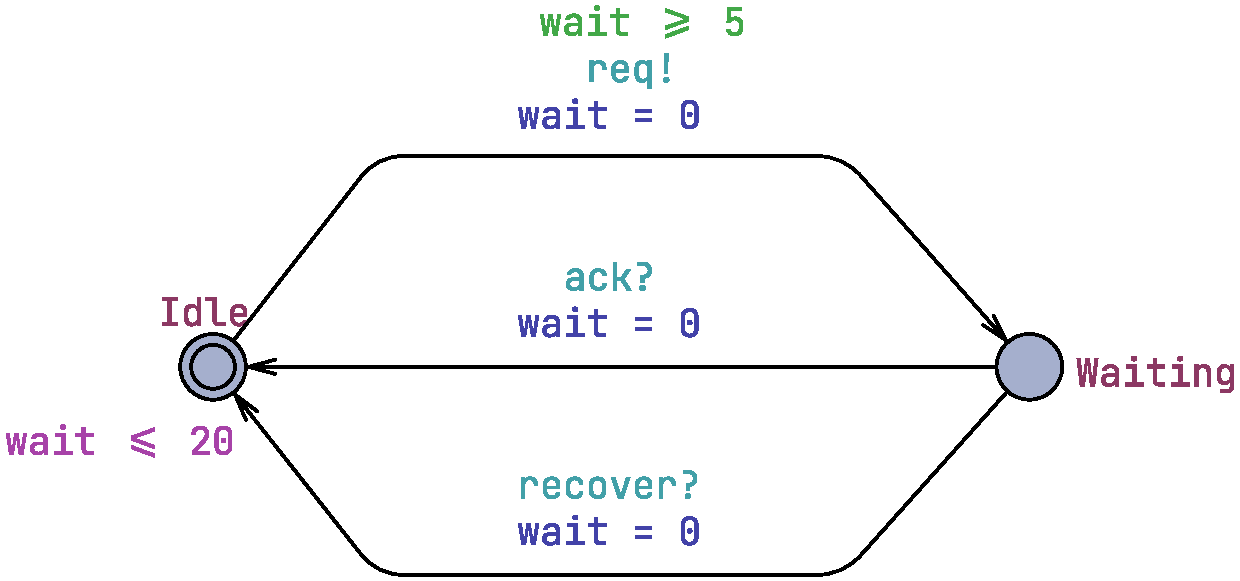
\includegraphics[width=0.58\columnwidth]{figures/gear_shift_nta_Driver-cropped.pdf}\\[-0.35em]
  {\footnotesize (a) Driver}\\[0.2em]
  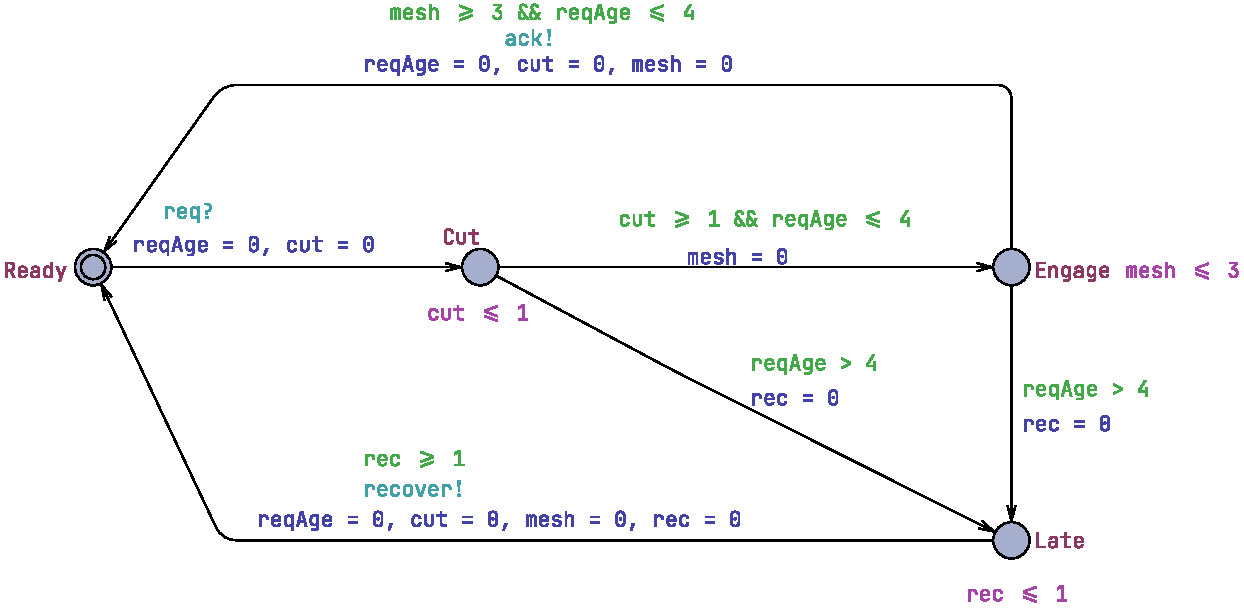
\includegraphics[width=0.98\columnwidth]{figures/gear_shift_nta_GearController-cropped.pdf}\\[-0.55em]
  {\footnotesize (b) GearController}
  \caption{Simplified gear-shift example.}
  \label{fig:gear-shift-nta}
  \vspace{-0.5em}
\end{figure}

\noindent\textit{Example 1.}
Figure~\ref{fig:gear-shift-nta} shows the running gear-shift example.
The Driver issues a request through $\mathit{req}!$, and the controller
responds through $\mathit{ack}!$ or $\mathit{recover}!$. In the faulty
controller, $\mathit{cut}\leq 1$ and $\mathit{cut}\geq 1$ allow
engagement after one time unit, violating property $\varphi_1$, which
requires at least two time units of torque cut. A single-property repair
can change these bounds to $2$. However, if the
$\mathit{mesh}\leq 3$ and $\mathit{mesh}\geq 3$ bounds remain unchanged,
the earliest acknowledgement occurs after $2+3=5$ time units, violating
property $\varphi_2$, which requires acknowledgement within four time
units. A multi-property repair must therefore adjust both
$\mathit{cut}$ and $\mathit{mesh}$ while preserving the original
functional behavior, including the request--engage--acknowledge path.

TDTs provide concrete realizations of property violations, but they do
not explain why the violations occur. In particular, a TDT does not
identify which numerical bound is faulty or whether the relevant bound
appears in a guard or an invariant. Following the idea of TARTAR
\cite{kolbl2019clock}, the repair procedure developed later in this
paper encodes TDTs as arithmetic constraints over trace feasibility,
property violation, and bound variations. Unlike single-property repair,
MPTA-Repair organizes constraints from multiple violated properties and
TDTs into a joint solving process to generate candidate clock-bound
repairs.

Let $M_{\mathit{bad}}$ be a faulty NTA model and let
$\Phi=\{\varphi_1,\ldots,\varphi_m\}$ be the set of properties that must
be satisfied simultaneously. MPTA-Repair generates a repaired model
$M_{\mathit{rep}}$ by changing repairable numerical bound occurrences
in guards and invariants. A candidate repair is accepted only if
\begin{equation}
  M_{\mathit{rep}}\models \bigwedge_{\varphi\in\Phi}\varphi
  \quad\land\quad
  \mathrm{Accept}(M_{\mathit{bad}},M_{\mathit{rep}}).
\end{equation}
The first condition requires the repaired model to satisfy all required
properties. The second condition denotes a TARTAR-style admissibility
check based on functional equivalence~\cite{kolbl2019clock}. This check
prevents repairs that satisfy properties merely by disabling required
actions.

\section{Approach}
\label{sec:approach}

\subsection{Overview}

MPTA-Repair is a counterexample-guided framework designed for the
multi-property clock-bound repair of timed automata models. The
framework takes as input a faulty model $M$, a property set
$\Phi=\{\varphi_1,\ldots,\varphi_m\}$, and configuration parameters such
as a global timeout. Instead of requiring users to manually specify
repair variables, MPTA-Repair extracts repairable bounds from numerical
clock constraints in transition guards and location invariants. The
output is either a repaired model $M'$ along with a set of clock-bound
edits, or a failure report indicating that no admissible full-property
repair was identified within the given time budget.

MPTA-Repair is based on two observations. First, while candidate repair
generation can be driven by local diagnostic traces, candidate
validation must remain global. A candidate that repairs one violated
property might induce failures in others, because shared clocks,
locations, transitions, or synchronizations often participate in
multiple timing requirements. Consequently, MPTA-Repair iteratively
collects counterexamples from subsequent violations to progressively
constrain the space of admissible repair candidates. This refinement
loop continues until a candidate satisfies the entire property set and
passes admissibility verification, or the given time budget is
exhausted.

Second, different properties and diagnostic traces are often related
through shared repairable bounds. A single erroneous timing bound can
contribute to multiple violations, and distinct traces may correspond to
different executions of the same underlying fault. To leverage this
interdependence, MPTA-Repair maintains a joint pool of property-trace
obligations and searches for a clock-bound assignment that
simultaneously satisfies all encoded constraints while minimizing the
total modification cost. Relational analysis across properties, traces,
and repairable bounds serves to minimize redundant computations and
guide the search space exploration, though the generated candidates must
ultimately pass verification and admissibility checks.

In operation, MPTA-Repair initially verifies the model against the
property set and collects timed diagnostic traces (TDTs) for any
violations. It then extracts repairable clock bounds and constructs a
joint MaxSMT repair problem from the active property-trace pool. The
computed assignment is instantiated into a candidate model, which
undergoes validation against the complete property set and a
functional-equivalence admissibility criterion. If validation fails,
newly identified diagnostic traces are integrated into the pool, and the
refinement loop repeats.

Figure~\ref{fig:mpta-repair-workflow} illustrates the overall workflow.
The initial verification stage populates the property-trace pool.
Subsequently, the relation-guided optimization phase structures the
dependencies among properties, counterexamples, and repairable bounds.
Finally, the MaxSMT solving stage generates candidate edits. The
validation component either accepts an admissible repair or feeds new
diagnostic evidence back into the subsequent refinement round.

\begin{figure*}[t]
  \centering
  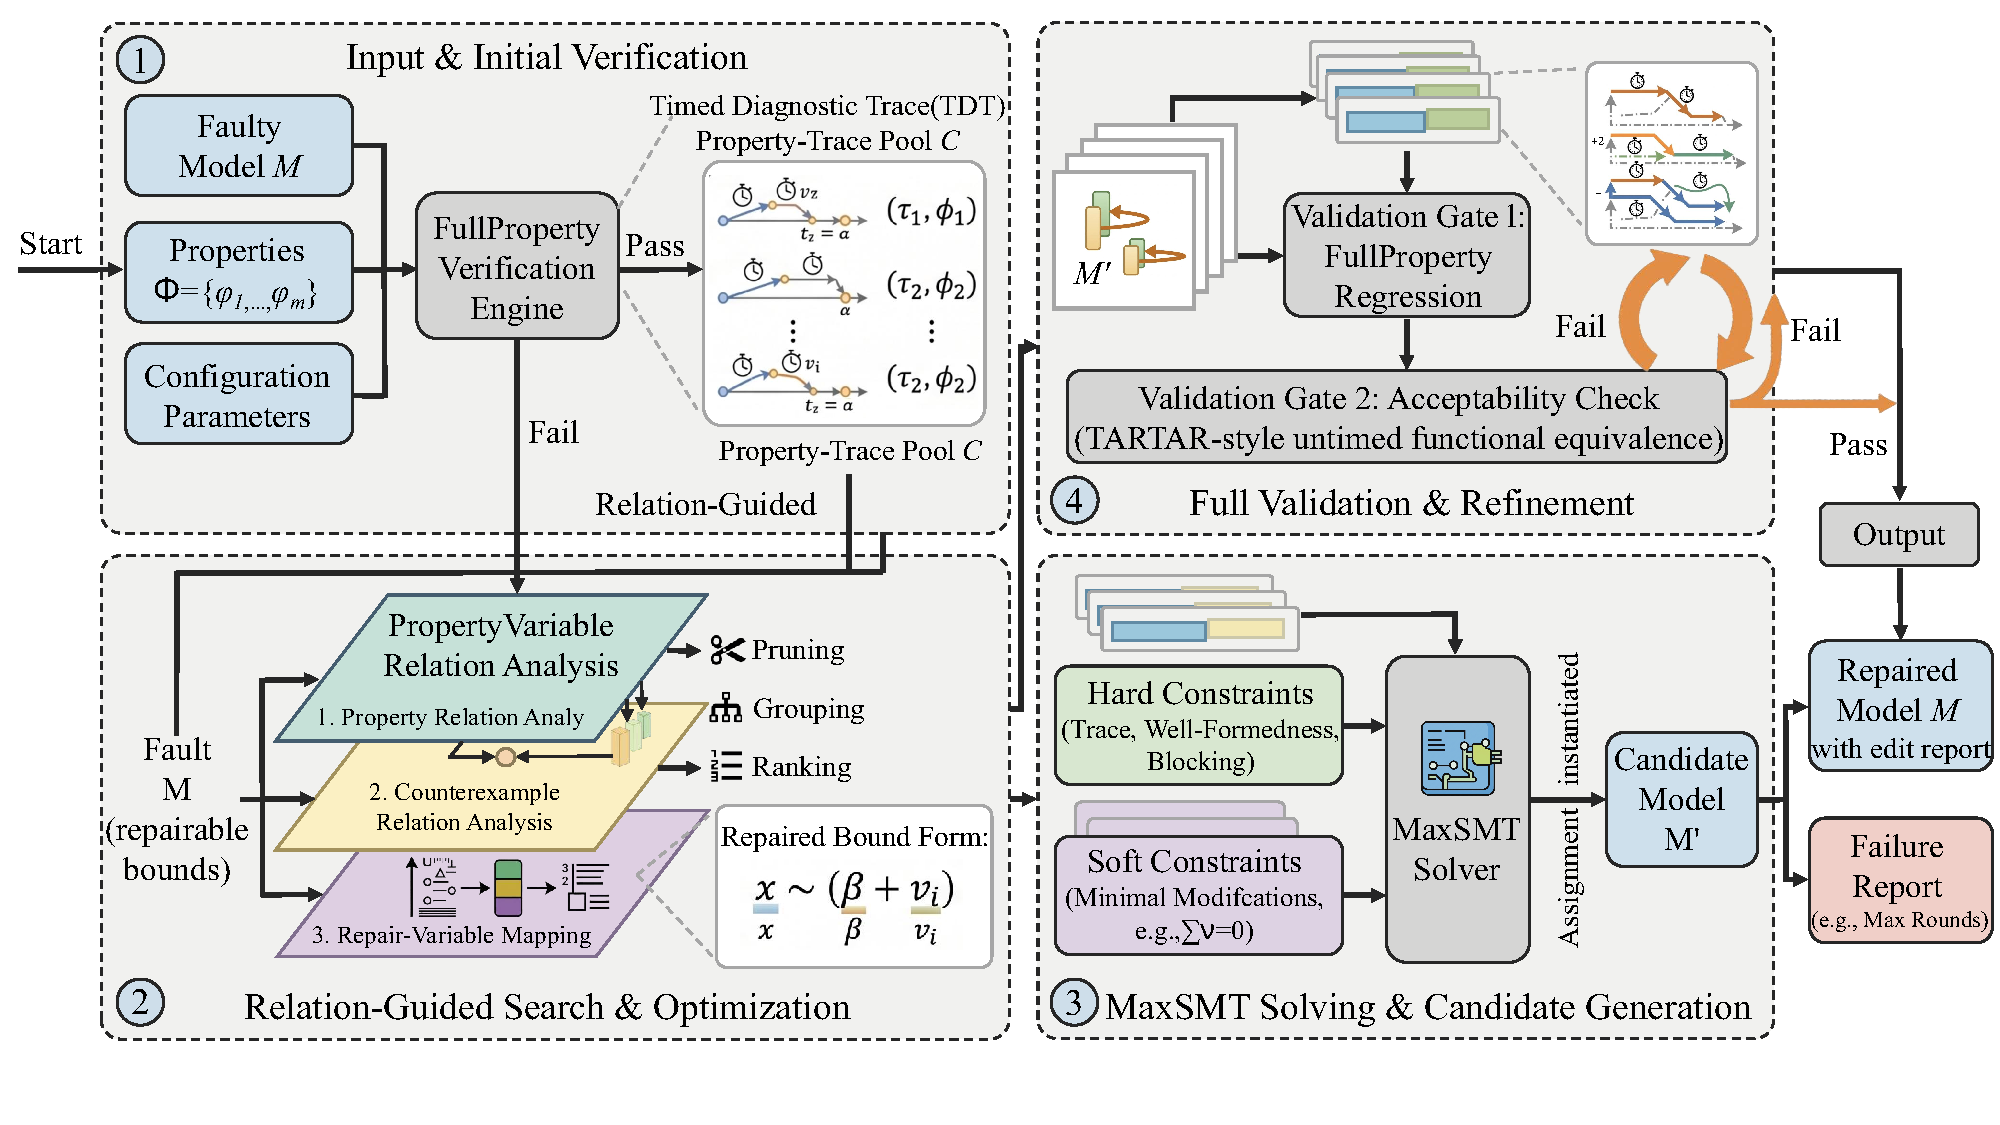
\includegraphics[width=0.98\textwidth]{mpta_repair_framework.pdf}
  \caption{Overview of the MPTA-Repair workflow.}
  \label{fig:mpta-repair-workflow}
\end{figure*}

\subsection{Joint Trace Encoding and Optimization Objective}

MPTA-Repair adopts the bound-variation paradigm for clock-bound repair
\cite{koelbl2019clock}. Each modifiable numerical bound in a transition
guard or location invariant is associated with a variation variable,
ensuring that the repaired constraint retains the original clock
reference and comparison operator while incorporating a shifted
numerical value. Consequently, the repair space is restricted to
clock-bound constants, whereas transition structures, location
topologies, synchronization labels, reset sets, and discrete updates
remain unaltered.

For each diagnostic trace, the framework constructs a TARTAR-style trace
constraint system \cite{koelbl2019clock} encompassing standard
conditions for clock initialization, time elapse, clock resets, guard
satisfaction, and invariant satisfaction. By replacing original clock
bounds with their varied counterparts, this formulation preserves the
discrete trace skeleton within the solver while allowing its timing
region to change. For a violated property and diagnostic trace, the
resulting obligation serves two purposes. It ensures post-repair
executability of the discrete trace skeleton to prevent trivial
elimination of functional paths, and it requires that no feasible timing
realization of this skeleton violates the target property. Local
obligations therefore isolate violating timed behaviors without blocking
the underlying functional execution.

To guarantee physical validity during candidate generation, static
consistency constraints are embedded directly into the formulation
\cite{demoura2008z3}. Repaired bounds must lie within the supported
numerical domain. Furthermore, when a lower bound and an upper bound
jointly constrain the same clock within a local region, their repaired
values must maintain a consistent timing interval.

From the active pool of property-trace obligations, MPTA-Repair
assembles a joint MaxSMT problem. The hard constraints include all
encoded trace obligations, static consistency requirements,
well-formedness conditions for repaired bounds, and blocking constraints
derived from previously rejected candidates. The optimization objective
is governed by a hierarchical set of simple soft constraints
\cite{sebastiani2015optimization}. The primary objective minimizes the
number of altered clock bounds by maximizing soft constraints of the
form $v=0$. Among candidate solutions with the same number of
modifications, a secondary objective minimizes the total magnitude of
the variations. This optimization strategy aligns with the engineering
goal of generating minimal, human-inspectable repairs and deliberately
avoids speculative metrics such as semantic risk or causal relevance.
Relation analysis is instead used externally to select or rank repair
variables and obligations before and around the solving phase.

\subsection{Relation-Guided Search Optimization}

During successive refinement rounds, the accumulation of violated
properties, diagnostic traces, and editable clock bounds can
significantly expand the search space \cite{clarke2000cegar}.
Unstructured encoding of all property-trace obligations and repairable
bounds increases the complexity of the MaxSMT problem and can induce
redundant solving cycles over overlapping evidence. To mitigate this
overhead, MPTA-Repair introduces relation-guided optimization to prune,
group, and rank variables and constraints. These relation-based
heuristics serve strictly as search optimizations; validity and
admissibility of generated candidates are still guaranteed through
full-property regression and formal verification.

At the property layer, MPTA-Repair operates on safety properties
normalized into an $\mathtt{A}[]$ fragment over location predicates and
clock or integer constraints \cite{vogel2022patterns}. Relation analysis
uses conservative syntactic and structural rules to evaluate equivalence
and dominance. Two properties are equivalent only when their normalized
representations are syntactically identical. Dominance is established
only when clear logical subsumption holds, for example when two
upper-bound properties share identical structures but differ in their
numerical thresholds and one threshold strictly implies the other.
Shared clocks, target locations, and template structures are tracked as
dependency metadata, but they do not independently justify removing
obligations.

At the counterexample layer, the framework maintains a managed pool of
TDTs indexed by their corresponding violated properties. Redundant
traces are eliminated through exact-duplicate removal. The remaining
TDTs are annotated with structural features, including traversed
transitions, visited locations, active clocks, guard and invariant
bounds, and originating properties \cite{koelbl2019clock}. Structural
similarity, common prefixes, and shared repair variables are used to
cluster related traces and orchestrate joint solving. A trace obligation
is deactivated only when an exact duplicate is detected or when a sound
subsumption check proves that its local constraint profile is covered by
an existing encoded obligation.

At the repair-bound layer, MPTA-Repair establishes a mapping between
each active property-trace obligation and the clock bounds capable of
influencing its feasibility. This mapping restricts the active decision
variables in the MaxSMT problem to those directly relevant to the
current counterexample pool, while providing a heuristic ordering for
candidate generation. Rather than imposing rigid structural constraints
or hard-coding specific modifications, relation scores serve as an
adaptive guidance mechanism. They improve search efficiency by
dynamically deactivating irrelevant repair variables, ensuring that the
solver concentrates on dimensions supported by counterexample evidence.

\subsection{Validation, Admissibility, and Refinement}

Candidate validation serves as the primary correctness guarantee in
MPTA-Repair \cite{clarke1999model}. After a candidate edit set is
generated, the repaired model is verified against the entire property
set $\Phi$. If a candidate resolves the triggering violation but
introduces a failure in another property, it is rejected, indicating
that the current property-trace pool is under-constrained. MPTA-Repair
then extracts the newly observed diagnostic trace and appends it to the
pool, steering the subsequent refinement round.

Candidates that pass full-property regression are further evaluated
against a TARTAR-style admissibility criterion based on functional
equivalence \cite{koelbl2019clock}. This step ensures that clock-bound
modifications do not satisfy safety properties by disabling intended
system behaviors. Rather than enforcing timed-language equivalence,
which would conflict with the goal of eliminating violating timed paths,
admissibility is checked by constructing untimed automata from both the
original and repaired models and comparing their accepted untimed
languages \cite{hopcroft2001automata}. A candidate is rejected if it
adds or removes discrete functional paths, ensuring that only timing
characteristics are changed.

The refinement loop therefore establishes a closed-loop mechanism that
pairs local candidate generation with global validation. Local MaxSMT
formulations propose candidate assignments, full-property regression
ensures complete specification compliance, and functional-equivalence
checking preserves the underlying discrete structure. Blocking
constraints prevent recurrence of failed assignments, ultimately
yielding a repair that satisfies the multi-property specification while
preserving the intended untimed model semantics.

\section{Experimental Evaluation}
\label{sec:evaluation}

This section evaluates MPTA-Repair on both benchmark and industrial
case studies. The evaluation follows the clock-bound repair setting
defined in Section~\ref{sec:approach}, where only numerical bounds in
guards and invariants are repairable. Comparing MPTA-Repair with an
iterative baseline extended from the TARTAR paradigm
\cite{leue2019clock} demonstrates that multi-property regression and
multi-counterexample analysis are essential to prevent secondary
property violations.

\subsection{Evaluation Strategy and Datasets}

We evaluate MPTA-Repair on two datasets, summarized in
Table~\ref{tab:dataset-statistics}. The benchmark dataset includes nine
standard models from UPPAAL \cite{behrmann2004tutorial} and the
XtaBenchmarkSuite \cite{farkas2018benchmarks}, such as Elevator and
FDDI. The industrial dataset contains five closely coupled industrial
case studies: Gear Control System for automotive transmission
\cite{lindahl1998gear}, SAE RoR for autonomous-driving decisions
\cite{alves2021double}, Train Controller Alarm for railway emergency
timing \cite{gonzalez2024uppaal}, Train Gate Controller for
shared-resource concurrency \cite{alur1994theory}, and Pacemaker for
medical device pacing \cite{jiang2010heart}. Compared with the
benchmark models, these case studies involve more tightly coupled
timing constraints across multiple properties.

\begin{table}[t]
\caption{Statistics of the benchmark and industrial datasets.}
\label{tab:dataset-statistics}
\centering
\scriptsize
\setlength{\tabcolsep}{2pt}
\begin{tabular*}{\linewidth}{@{\extracolsep{\fill}}lccccc@{}}
\toprule
Dataset & Original models & Mutated models & Avg. properties/model &
Avg. loc. & Avg. trans. \\
\midrule
Benchmark & 9 & 54 & 4.1 & 30.56 & 52.67 \\
Industrial & 5 & 105 & 7.3 & 57.80 & 91.80 \\
\bottomrule
\end{tabular*}
\end{table}


Since real-world timed-automata models with labeled clock-bound faults
are difficult to obtain, we synthesize faulty instances using mutation
\cite{jia2011mutation}. We retain only mutants that are syntactically
valid, violate at least one timing safety property, and preserve the
untimed behavior of the original model.

We compare MPTA-Repair against an adapted iterative TARTAR-style
baseline \cite{leue2019clock}. Because the TARTAR method was originally
designed for single-property repair and lacks joint multi-counterexample
relation analysis, this comparison allows us to examine whether using a
joint counterexample pool improves repair robustness over trace-local
repair generation. The comparison is designed to evaluate the effect of
jointly analyzing properties, counterexamples, and repair variables.

\subsection{Experimental Results}

The experimental evaluation demonstrates that MPTA-Repair outperforms
the iterative baseline, particularly on complex industrial models. As
shown in Table~\ref{tab:overall-results}, the baseline achieves a 72\%
success rate on the benchmark dataset, whereas MPTA-Repair reaches
93\%. This performance gap widens on the industrial dataset, where the
baseline repairs only 20\% of the cases compared to 76\% for
MPTA-Repair. These results indicate that our approach remains effective
on standard timed-automata benchmarks while demonstrating robustness in
complex industrial systems where properties and traces interact closely.
The average repair time should be interpreted together with the success
counts. On the industrial dataset, the iterative baseline has a lower
average time because many cases fail quickly, not because it repairs
industrial models more efficiently.

\begin{table}[t]
\caption{Repair success rates across benchmark and industrial datasets.}
\label{tab:overall-results}
\centering
\scriptsize
\setlength{\tabcolsep}{4pt}
\begin{tabular*}{\linewidth}{@{\extracolsep{\fill}}llc@{}}
\toprule
Dataset & Method & Success rate \\
\midrule
Benchmark & Iterative baseline & 72\% \\
Benchmark & MPTA-Repair & 93\% \\
Industrial & Iterative baseline & 20\% \\
Industrial & MPTA-Repair & 76\% \\
\bottomrule
\end{tabular*}
\end{table}


The baseline is competitive on simpler benchmark models because timing
errors are frequently concentrated on isolated guards or invariants. In
these localized scenarios, a single diagnostic trace often provides
sufficient information to infer a correct repair. However, even within
standard benchmarks featuring shared multi-channel structures, such as
the FDDI protocol, MPTA-Repair is more robust because it prevents
single-trace overfitting. This advantage becomes more pronounced in
complex industrial models that feature interacting concurrent
components, urgent or broadcast synchronization channels, observer
templates, and array-based constructs. In these settings, localized
repairs by the baseline frequently fail subsequent global validation
checks. Our empirical analysis shows that the baseline lacks explicit
optimization to minimize edit magnitude, often generating extreme
candidate bounds that violate admissibility. Additionally, the baseline
struggles with regression verification over three to nine coupled
properties because it does not analyze their corresponding
counterexamples jointly.

MPTA-Repair achieves higher success rates due to two primary design
advantages. First, multi-counterexample accumulation reduces overfitting
to a single timed diagnostic trace, which typically exposes only one
timing realization of an underlying fault. By accumulating and analyzing
diagnostic traces from multiple operational modes, the framework
synthesizes minimal joint edit sets that address the timing fault
comprehensively. Second, relation-guided optimization complements
precise MaxSMT objectives to improve candidate quality. By identifying
diagnostic traces that share path fragments or target repair variables,
the solver focuses on modifying numerical clock bounds close to the
observed violations while penalizing large edit magnitudes. Successful
repairs therefore typically require modifying only one or two critical
clock bounds, which facilitates subsequent manual inspection and
verification.

\subsection{Discussion and Practical Lessons}

The evaluation highlights several insights for applying automated repair
to industrial timed automata. First, full-property regression testing is
necessary. Because industrial system properties are interdependent, a
localized fix designed solely to satisfy a liveness-like response
monitor can inadvertently violate a separate safety monitor that
constrains maximum waiting times. MPTA-Repair avoids these behavioral
regressions by treating overall property restoration as a global
objective. Second, admissibility is critical to measuring repair
success. Without ensuring structural and functional equivalence, a
solver might satisfy a specific timing property by disabling the
intended functional behavior, such as preventing a critical system
action entirely. The strict admissibility check ensures that property
satisfaction is not achieved at the expense of untimed functional
behavior.

Our failure analysis reveals several limitations of the current repair
space. Computational timeouts and unsupported model syntax account for
only a portion of the unsuccessful repair attempts. In tightly coupled
domains such as cardiac pacing, certain complex errors require
simultaneous, consistent adjustments across both guards and invariants,
which significantly expands the search space. Additionally, incomplete
diagnostic trace coverage from the verification engine can occasionally
lead to overfitting. Certain complex cases lacked any feasible candidate
within the restricted clock-bound parameter space. This limitation
suggests that repairing these models requires broader structural
modifications, such as altering synchronization labels, adjusting clock
resets, or modifying discrete data updates.

\section{Threats to Validity}
\label{sec:threats}

\textbf{Internal validity.} The prototype includes parsers for
NTA models, property files, diagnostic traces, repair sites,
and admissibility artifacts. Bugs in parsing, trace reconstruction, SMT
encoding, candidate application, or admissibility checking may affect
the results. We mitigate this threat by validating every accepted
candidate using the external model checker and by recording repair
reports for each run.

\textbf{Construct validity.} The evaluation uses injected clock-bound
faults. Such faults are appropriate for evaluating clock-bound repair,
but they do not cover all real modeling errors. Real faults may involve
wrong resets, missing transitions, incorrect synchronizations, data
updates, or erroneous properties. The results should therefore be
interpreted as evidence for clock-bound repair, not for arbitrary NTA
repair.

\textbf{External validity.} Although the industry dataset covers several
practical domains, it is still a finite set of open or reconstructed
models. It may not represent all industrial NTA models.
Larger proprietary models, richer data variables, and more complex
property specifications may introduce additional challenges.

\textbf{Baseline fairness.} The baseline is an iterative TARTAR-style
repair workflow adapted to the multi-property setting by adding
full-property regression and admissibility checking. This makes it
stronger than a one-shot baseline, but it is still not identical to the
original setting for which TARTAR was designed. We therefore interpret
the comparison as a comparison against a strong single-property repair
strategy, not as a claim that TARTAR itself is unsuitable in general.

\textbf{Property selection.} Industry-case properties were selected from
model descriptions, papers, embedded queries, and intended timing
requirements. Some properties may be incomplete or may not capture all
domain-level requirements. We mitigate this by requiring all reference
models to satisfy the selected property set and by filtering out trivial
guard-mirror properties when constructing the benchmark.

\textbf{Repair-space limitation.} The current method focuses on
numerical clock-bound edits in guards and invariants
\cite{kolbl2019clock}. Some failed cases likely require repair actions
outside this space. Extending the method to reset repair,
synchronization repair, clock-reference repair, and structural repair is
left for future work.

\section{Related Work}
\label{sec:related-work}

The closest related work is clock-bound repair for timed systems and
TarTar \cite{koelbl2019clock}. Clock-bound repair encodes timed diagnostic traces into
linear real arithmetic and uses MaxSMT solving to compute small
modifications to guard and invariant bounds \cite{koelbl2019clock}. TarTar extends this
line into a repair analysis tool and introduces an admissibility check
based on functional equivalence. MPTA-Repair builds on this foundation,
but targets a different setting: multiple properties, multiple
diagnostic traces, and full-property validation in timed-automata
models from practical industrial cases.

A second related direction is parameter synthesis for parametric timed
automata \cite{alur1993parametric}. Tools such as IMITATOR synthesize parameter valuations
that satisfy timing constraints or preserve behavior around a reference
valuation \cite{andre2010imitator}. These techniques are powerful for design-space
exploration and robustness analysis \cite{bendik2021robustness}. MPTA-Repair differs in its
use of diagnostic traces and its focus on producing small syntactic
repairs for faulty models rather than synthesizing a full parameter
region.

A third related direction is model repair and automated program repair
using SAT, MaxSAT, SMT, and counterexample-guided refinement \cite{weimer2009automatically}.
These works provide search and optimization ideas such as fault
localization \cite{jose2011bugassist}, candidate blocking \cite{mechtaev2016angelix}, repair minimization
\cite{nguyen2013semfix}, and abstraction refinement \cite{clarke2000cegar}. MPTA-Repair adapts this
style of reasoning to the semantics of timed automata, where candidate
validity must consider both timing properties and untimed behavior
preservation.

Finally, this work is related to industrial verification and
dependability engineering \cite{leveson2011safer}. Industry-oriented verification often
emphasizes full regression, explainability, traceability, and lessons
learned rather than only theoretical completeness \cite{clarke2018handbook}. MPTA-Repair
follows this perspective by treating repair as an engineering workflow:
diagnostic traces generate candidates, but acceptance depends on full
regression evidence and admissibility.

\section{Conclusion}
\label{sec:conclusion}

This paper presented \textbf{MPTA-Repair}, an automated workflow for
multi-property and multi-counterexample clock-bound repair of
industrial timed automata. To overcome the limitations of isolated
single-trace fixes, the method accumulates diagnostic traces and
exploits explicit relations among properties, counterexamples, and
repairable bounds to guide a MaxSMT-based search. Each synthesized
candidate is validated through full-property regression and an
admissibility check based on untimed functional equivalence
\cite{kolbl2019clock}. This design ensures that accepted repairs are
system-level timing corrections that preserve the intended operational
behavior.

Evaluations across benchmark and industrial datasets show that
MPTA-Repair outperforms the iterative baseline, particularly in
industrial systems with dense property interactions. The failure
analysis further indicates that unsuccessful repairs often stem from
the intrinsic limits of a strictly parametric clock-bound repair space.

Future work will primarily focus on extending the automated repair space
beyond numerical clock bounds to include broader structural
modifications, such as altering synchronization labels and redesigning
discrete control logic. We also plan to investigate the theoretical and
algorithmic relationship between candidate repair generation and
admissibility verification. By formally integrating behavioral
admissibility constraints into the early stages of search-space
formulation, we aim to proactively prune functionally invalid candidates
and thereby improve computational efficiency for large-scale industrial
applications.

\bibliographystyle{IEEEtran}
\bibliography{refs}
\end{document}
